\documentclass[12pt, letterpaper]{article}
\usepackage{graphicx}
\usepackage{fontenc}
\begin{document}
\title{Microscopic Traffic Flow Model}
\author{Prakhar Gupta - 2103126}
\thanks{wikipedia, }
\maketitle
Traffic flow is the study of interactions between travellers (like cars, trucks, buses, cyclist, pedestrians) and infrastructure (like highways, traffic stop, turns) with the purpose of understanding and developing an optimal network for efficient movement of traffic and minimal traffic congestion problems.

Traffic behaves in a complex and non linear way, depending upon interactions of large number of vehicles. Traffic flow theory refers to steam variables of speed, flow and concentration.

Terms:

Speed: It is the distance covered per unit time.
To get average speed of vehicles, there are two types of speed average - \begin{itemize}
\item Time mean speed 
	 Instantaneous speed of different vehicles is measured at a point on path. Then average of that speed is taken.
\item Space mean speed
	A snapshot of track is taken for getting speed of all vehicles at same time. Average of those speed is taken to get space mean speed.
\end{itemize}

Density: It is defined as the number of vehicles per unit length of the roadway. In traffic flow critical density and jam density are the most important density which describe a lot about a system.

Flow: It is the number of vehicles passing a reference point per unit of time (vehicles per hour). 

Methods of Analysis:
\begin{enumerate}
\item Microscopic Scale
Most basic level. Every vehicle is considered as individual. Equations (ODE- Ordinary Differential Equation) for each individual can be written and their nature can be deduced.
\item Macroscopic Scale
Advanced level where system as a whole is considered. It is considered useful to employ a system of partial differential equations, which gives quantities of interest; e.g., the density of vehicles or their mean velocity.
\item Mesoscopic Scale 
Intermediate between microscopic and macroscopic scale. Uses method of statistical mechanics.
\end{enumerate}
Microscopic Scale: 

In this level, individual vehicles are observed and data analysis is done in detailed level.

Our Model: Based on ''Follow the leader Theory''
\begin{itemize}
\item In our model we will consider a single lane and therefore no overtaking is allowed.
\item For driver behaviour and action we are using the `follow the leader' theory.
\item We are ignoring  traffic and road infrastructure like traffic lights, crossing, turns so as to keep our model simple and understandable.
\item We will also assume that no vehicles crash into each other and thus each vehicle maintains atleast some distance even in worst case scenerio.
\end{itemize}

\newpage
\includegraphics[]{traffic.jpeg}



\begin{equation}
x_{n-1} (t)= x_{n} + d + L_{n-1}      \textrm{\hspace{5pt} L represent the lenght of $n-1_{th}$ vehicle}
\end{equation} 
For n and n+1 vehicle.
\begin{equation}
x_n (t) - x_{n+1} (t) = d + L    \textrm{ \hspace{5pt} L represent the lenght of nth vehicle}
\end{equation} 
d is the separation between vehicles.

Leaders Model says :  Response  = Stimulus * Response time.

Stimulus for driver can be any or combination of these events
\begin{enumerate}
\item acceleration of vehicles
\item distance between vehicles
\end{enumerate}

In our model we incooperate the acceleration of vehicles as stimulus for response that will then act as stimulus for preceding vehicles and so on.

\begin{equation}
 \triangle x_{n+1} ^t = \triangle x_{safe} + \tau v_{n+1 }^t
 \end{equation}
 
$\triangle x_{n+1}$  denotes the gap between $ n+1^{th} $vehicle and $ n^{th}$ vehicle.
 $\triangle x_{safe}$
  denotes the least distance or gap that should be present even when the presiding vehicle is faster than successive vehicle.$v_{n+1} ^t $denotes the speed of $ n+1^{th}$ vehicle.$\tau$ is the sensitivity according to which $n+1^{th}$ vehicle adjust its speed.
 
 Therefore now we have:
 \begin{equation}
 x_n ^t - x_{n+1 } ^t = \triangle x_{safe} + \tau v_{n+1} ^t
 \end{equation}
 
 Differentiating the above equation with respect to time, we get
 \begin{equation}
 v_n ^t - v_{n+1 }^t = \tau a_{n+1 }^t
 \end{equation}
  \begin{equation}
 a_{n+1 }^t = \frac{1}{\tau} [v_n ^t - v_{n+1} ^t]
  \end{equation}
 
Thus our final equation is
 
 \begin{equation}
 \frac{d^2 x_{n+1} ^t}{dt^2} = \frac{1}{\tau} [\frac{d x_n ^t}{dt} - \frac{d x_{n+1} ^t}{dt}]
\end{equation}

Observations :

\begin{itemize}
\item Resultant equation is an ODE (ordinary differential equation) with order 2.
\item $\frac{1}{\tau} $ is sensitivity constant
\item If $\frac{d x_n}{dt} > \frac{d x_{n+1}}{dt}$
Leader is faster.
Follower would accelerate.

Therefore $\frac{1}{\tau} > 0$

\item If $\frac{d x_n}{dt} < \frac{d x_{n+1}}{dt}$
Leader is slower.
Follower would deaccelerate.

Therefore$ \frac{1}{\tau}  > 0$

\item This ODE is difficult to solve because acceleration of each vehicle is dependent on vehicle successive to it. Thus we need to solve n ODE to get acceleration and velocity of n+1 vehicle.
\end{itemize}

Speed density Relationship -
\begin{equation}
\frac{d x_{n+1} ^t}{dt ^t} = \int \frac{ d^2 x_{n+1} ^t}{dt^2}
\end{equation}
\begin{equation}
 \frac{d^2 x_{n+1} ^t}{dt^2} = \frac{1}{\tau} [\frac{d x_n ^t}{dt} - \frac{d x_{n+1} ^t}{dt}]
 \end{equation}
 
 Using (8) and (9)  we get
 \begin{equation}
 \frac{d x_{n+1} ^t}{dt} = \int \frac{1}{\tau} [\frac{d x_n ^t}{dt} - \frac{d x_{n+1} ^t}{dt}]
 \end{equation}
 Integrating the above equation with respect to t:
\begin{equation}
  \frac{d x_{n+1} ^t}{dt} =  \frac{1}{\tau}[  x_n ^t -  x_{n+1} ^t] + c_{n+1} 
  \end{equation}
 \begin{equation}
 v_{n+1} ^t =   \frac{1}{\tau}[  x_n ^t -  x_{n+1} ^t] + c_{n+1} 
  \end{equation}
  Speed of $n+1_{th}$ is dependent on space ahead of it.

Also:  
\begin{equation}
v_{avg} =  \frac{\sum _1 ^N v_n}{N}  \textrm{\hspace{5pt}where N is the total number of vehicles}
\end{equation}
 
 Therefore (12) can be written as:
 \begin{equation}
 v_1 ^t + v_2 ^t + v_3 ^t + \cdots + v_{n+1} ^t = \frac{1}{\tau} [(x_0 ^t  - x_1^t) + (x_1 ^t - x_2 ^t) + \cdots + (x_n ^t + x_{n+1} ^t)] + c'
 \end {equation}  
 \begin{equation}
 \frac{ v_1 ^t + v_2 ^t + v_3 ^t + \cdots + v_{n+1} ^t }{N} = \frac{\frac{1}{\tau} [(x_0 ^t  - x_1^t) + (x_1 ^t - x_2 ^t) + \cdots + (x_n ^t + x_{n+1} ^t)]} {N} + c''
 \end{equation}
 \begin{equation}
 v_{avg} = \frac{1}{\tau} \frac{[x_0 ^t - x_{n+1} ^t]}{N} + c''
  \end{equation}
  
  As space between $0_{th} $ vehicle and $n_{th}$ represent the path lenght ,
  thus $ \frac{[x_0 ^t - x_{n+1} ^t]}{N} $ = L .  L is the path length or road segment we have taken is consideration.
  
  Also $\frac{N}{L} = \rho$ where $\rho$ is the linear density of path or road. Linear density is defined as number of vehicles per unit length.
  
  \begin{equation}
  v_{avg} = \frac{1}{\tau \rho} + c''
  \end{equation} 
 
To get value of c'' ,  we set condiction that at $\rho_{max}$ , $v_{avg}$ = 0
  
 Therefore speed-velocity relationship equation:
  \begin{equation}
  v_{avg} = \frac{1}{\tau}[\frac{1}{\rho} - \frac{1}{\rho_{max}}]
  \end{equation}
  
Observation:
\begin{itemize}
\item $\frac{dv_{max}}{d\rho}$ = $\frac{1}{\tau} (-\frac{1}{\rho ^2})$
\item $\rho$ = $\rho_{max}$ then $v_{avg} ^t$ = 0
\item $\rho = 0 $, $v_{avg} ^t= \infty$
\end{itemize}

The third observation gives room for improvement in speed-velocity equation as when $ \rho = 0$, $v_{avg} = v_{max}$

Finalized speed-velocity equation:
 \begin{equation}
  v_{avg} = \frac{1}{\tau}[\frac{1}{\rho} - \frac{1}{\rho_{max}}]   \textrm{ when $\rho > \rho_{critical}$}
    \end{equation}
     \begin{equation}
  v_{avg} = v_{max} \textrm{ when $\rho < \rho_{critical}$}
  \end{equation}

Graph of avg velocity vs density :

 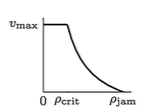
\includegraphics[]{C:/Users/Prakhar/Desktop/flow.png}
 
 Flow density relationship - 
 
 q (Flow) = $\rho \times  v$
 
 Therefore 
 \begin{equation}
   q = \frac{1}{\tau}[1 - \frac{\rho}{\rho_{max}}]   \textrm{ when $\rho > \rho_{critical}$}
    \end{equation}
     \begin{equation}
  q = \rho  \times v_{max} \textrm{ when $\rho < \rho_{critical}$}
  \end{equation}
  
  At contant $v_{avg}$
  
  Graph of density vs flow
  
  
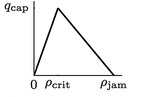
\includegraphics[]{C:/Users/Prakhar/Desktop/flow2.png}

Result:
\begin{itemize}
\item We solved a very simple model based on a real world complex network of traffic flow and arrived at an ODE.
\item That ODE, if solved for whole model will give property of each vehicle like their instanteous speed and acceleration at any time t.
\item Using ODE we found that speed density relationship and flow density relationship that better depicts of what happens in real world.
\item Even though our model is far too simple, still we get idea of how density of vehicles affect the number of vehicles passing per unit time (flow).  
\end{itemize}
Model Limitation:-
\begin {itemize}
\item Our model takes certain assumptions that deviate from real world like we assumed that sensitivity constant for each driver is same while in real world more experienced drivers have better sensitivity that less experienced ones.
\item Our model is a very simplisitic approach for a very complex real world problem. We did not take account for various infrastructure and surrounding that affect speed and density (like traffic light, crossroads, turns, u turns etc)
\item In our leader theory we took acceleration as the only stimulus that effect driver while in real world its not the only stimulus. 
\end{itemize}

 References:
\begin{itemize}
 \item https://www.civil.iitb.ac.in/tvm/1100\_LnTse/509\_lnTse/plain/plain.html
 \#:~:text=A\%20microscopic\%20model\%20of\%20traffic,different\%20features\%20of\%20a
 \%20road.
 
\item  https://en.wikipedia.org/wiki/Microscopic\_traffic\_flow\_model
\item https://en.wikipedia.org/wiki/Traffic\_flow
\item https://www.youtube.com/watch?v=4k-yIrPu5hA
\end{itemize}



\end{document}




